\chapter{attract mode admin}
\label{sec:attract_mode}
\lhead[tempest]{}
\lstset{style=6502Style}

There is naturally a bit of administrative overhead associated with operating
a game in 'attract mode'. In case you may be wondering, 'attract mode' is when a game cabinet
sits unattended and is attempting to attract customers. The manufacturer can display a colourful title
screen and high score tables, maybe play a tune. But often the most effective way of getting
people to play your game is to show the game being played. This allows the uninitiated to get a sense
of what they're missing out on and also gives them an idea of how to proceed when they
enter their first coin.
Providing this kind of demonstration gameplay means devising some rudimentary intelligence in the game logic that will
mimic the activity of a fairly competent paying customer. Fortunately, in \textit{Tempest}
there are only
two things that a player actually does: move and shoot. This means that our task of 
emulating a player negotiating a level in \textit{Tempest} is simpler
than it might at first appear. We can split it out into two separate concerns, and if we solve 
each one we will have an artificial player that can help bring in some business.

When we get our 'attract mode' up and running we have a small bit of setup to
perform first. The demonstration player is only given one life, and the level they
will play is chosen at random from the first eight.
\begin{lstlisting}
        BIT QSTATUS   ; CHECK FOR ATTRACT MODE..
        IFPL          ; IF IT IS ENABLED THEN..
        LDY I,1       ; LOAD 1 INTO Y REGISTER.
        STY LIVES1    ; AND STORE THAT AS AVAILABLE LIVES.
        LDA RANDOM    ; STORE A RANDOM NUMBER IN ACCUMULATOR.
        AND I,7       ; CLAMP IT TO BETWEEN 0 AND 7.
        ENDIF
        STA X,WAVEN1  ; USE THE RANDOM NUM TO SELECT LEVEL.
        STA CURWAV    ; STORE IT AS THE CURRENT LEVEL TOO.
\end{lstlisting}

With this environment for our player established we can first figure out how to make
him move.
\section*{movement admin}
This one is surprisingly easy. At any given moment we just have to decide whether
the cursor (representing the player) is going to move left or right. The only thing
that should ever affect this decision is whether the movement gets us nearer the same
line as the enemy that is nearest the top of the web. The diagram below shows this
decision-making in action. We are much nearer the line of the invader that is second
farthest away from us, but rather than move right towards that enemy, we move left:
towards the enemy that is closest to reaching the top of the web.

\begin{minipage}[c]{0.48\linewidth}
\begin{figure}[H]
    \centering
    \begin{adjustbox}{width=6cm,center}
      \includegraphics[width=3cm]{src/attractmode/movement_example1_before.png}%
    \end{adjustbox}
\end{figure}
\end{minipage}
\begin{minipage}[c]{0.06\linewidth}
\begin{figure}[H]
    \centering
    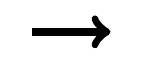
\begin{tikzpicture}[baseline={(current bounding box.south)}]
      \draw[->,line width=3pt] (0,0) to (1,0);
    \end{tikzpicture}
\end{figure}
\end{minipage}
\begin{minipage}[c]{0.48\linewidth}
\begin{figure}[H]
    \centering
    \begin{adjustbox}{width=6cm,center}
      \includegraphics[width=3cm]{src/attractmode/movement_example1_after.png}%
    \end{adjustbox}
\end{figure}
\end{minipage}

This approach, while it may be suboptimal in some ways, has the merit of being very
simple and we can implement it in a compact routine on the page opposite.

This routine consists of two steps. The first identifies the invader that has
advanced furthest along the web. The second then decides in which direction we must
move to get nearer to that invader. 

The first step is a simple matter of finding the invader with the highest 'Z Position' (which
is measured on the Y axis by \textit{Tempest} and stored in the \icode{INVAY} array for each
invader).
The second step depends on finding the shortest distance between the line the player's cursor is in and that
of the selected invader. A subroutine called \icode{POLDEL} is used to calculate this, and
the direction is indicated by whether the value is positive (to the left) or negative (to the right).
\clearpage
\begin{lstlisting}
  .SBTTL  PLAY-AUTO MOVE OF CURSOR
AUTOCU: 
  LDA I,-1        ; STORE -1 IN THE ACCUMULATOR.
  STA TEMP0       ; USE IT TO INITIALISE TEMP0.
  STA TEMP1       ; USE IT TO INITIALISE TEMP1.

  ; GET THE INDEX OF THE INVADER THAT IS FURTHEST ADVANCED
  ; ALONG THE WEB.
  LDX WINVMX      ; GET THE NUMBER OF INVADERS.
  BEGIN           ; LOOP FOR ALL INVADERS
    LDA X,INVAY   ; GET CURRENT INVADER'S DEPTH POSITION. 
    IFNE          ; IF IT HAS ONE THEN..
      CMP TEMP0   ; IS IT THE HIGHEST SO FAR?
      IFCC        ; IF IT IS THEN..
      STA TEMP0   ; STORE THE NEW HIGHEST POSITION.
      STX TEMP1   ; STORE THE INDEX OF HIGHEST INVADER.
      ENDIF
    ENDIF
    DEX           ; GO THE NEXT INVADER.
  MIEND           ; LOOP UNTIL WE'VE CHECKED THEM ALL.

  ; FIGURE OUT IF MOVING LEFT OR RIGHT GETS US NEARER TO THE
  ; FURTHEST ADVANCED INVADER.
  LDX TEMP1      ; STORE INDEX TO FURTHEST ADVANCED INVADER IN X.
  IFPL           ; IF WE FOUND ONE THEN..
    LDA X,INVAL1 ; GET THE LINE THE INVADER IS ON.
    LDY CURSL1   ; GET THE LINE THE PLAYER IS ON.
    JSR POLDEL   ; CALCULATE HOW FAR AWAY ONE IS FROM THE OTHER. 
    TAY          ; STORE THE RESULT IN Y REGISTER.
    IFNE         ; IF PLAYER IS NOT ALREADY ON SAME LINE AS ENEMY..
      IFPL       ; THEN IF RESULT FROM POLDEL IS POSITIVE..
      LDA I,-9   ; MOVE LEFT..
      ELSE       ; OTHERWISE..
      LDA I,9    ; MOVE RIGHT.
      ENDIF
    ENDIF
  ENDIF
  RTS
\end{lstlisting}

This isn't a perfect strategy, as we've already indicated. It means we potentially
move away from invaders that are nearer to our line of fire. But it does at least
ensure that we are always attempting to kill any enemy that is in danger of reaching
the top of the web and overrunning us.
\clearpage
\section*{shooting admin}
As long as we're trying to get nearer to the enemy that poses the most imminent danger,
we should also have a strategy for what we do when we get there. The obvious one is: shoot.
And that is indeed what we do, but with some latitude on top that improves our chances of 
killing any invader that happens to be in our field of fire. Our strategy for shooting,
therefore, will be to look at every enemy, and every shot fired by the enemy, and fire 
a shot in their direction if the line they are on is within two moves from our present position.

This means we will fire a shot along lines even when there isn't an enemy currently there (in the
hope that they might move there soon). It also means we no pay attention to how many shots we have
already fired or any consideration to whether it might be better to wait for a better opportunity.

\begin{figure}[H]
    \centering
    \begin{adjustbox}{width=9cm,center}
      \includegraphics[width=3cm]{src/attractmode/shooting_between.png}%
    \end{adjustbox}
    \caption*{Shooting when no one is there: an example of firing player charges when enemies are adjacent.}
\end{figure}

We implement this simple control logic in the same routine responsible for shooting charges
when the player presses the fire button: \icode{FIREPC}. 
\begin{lstlisting}
  .SBTTL PLAY - FIRE PLAYER CHARGE
FIREPC:
  LDA CURSL2                ; GET THE PLAYER'S LINE POSITION.
  IFPL                      ; NON-NEGATIVE MEANS THEY'RE ALIVE SO.. 
  LDA QSTATUS               ; CHECK WHETHER IN ATTRACT MODE..
  IFPL                      ; IF WE ARE THEN..
    LDA CURMOD              ; UNLESS WE'RE DROPPING, CURMOD WILL BE 0. 
    STA TEMP0               ; STORE AS OUR PROVISIONAL FIRE DECISION.

    ; LOOP THROUGH ALL INVADERS AND ALL SHOTS FIRED BY INVADERS TO LOOK
    ; FOR ANY ON A LINE NEAR TO THE PLAYER.
    LDX I,NICHARG+NINVAD-1  ; THE NUMBER OF INVADERS PLUS INVADER SHOTS.
    BEGIN                   ; LOOP THROUGH ALL INVADERS + INVADER SHOTS.
      LDA X,CHARY+NPCHAR    ; GET DEPTH OF CURRENT INVADER.
      IFNE                  ; IF NON-ZERO, IT IS IN PLAY SO..
        LDA X,CHARL1+NPCHAR ; GET THE LINE IT'S ON.
        SEC                 ; SET THE CARRY BIT BEFORE SUBTRACTING.
        SBC CURSL1          ; SUBTRACT PLAYER LINE FROM INVADER LINE.
        IFMI                ; IF NEGATIVE MAKE IT AN ABSOLUTE NUMBER..
        EOR I,0FF           ; BY X-OR'ING THE RESULT.
        CLC                 ; AND CLEAR THE CARRY BIT BEFORE..
        ADC I,1             ; ADDING 1 TO THE DIFFERENCE.
        ENDIF
        CMP I,2             ; COMPARE THE RESULT WITH 2..
        IFCC                ; IF THEY ARE LESS THAN 2 LINES APART THEN..
        INC TEMP0           ; SET TEMP0 SO THAT WE WILL FIRE A SHOT.
        ENDIF
      ENDIF
      DEX                   ; MOVE TO THE NEXT INVADER.
    MIEND                   ; LOOP UNTIL ALL INVADERS & SHOTS ARE DONE.
    LDA TEMP0               ; STORE OUR FIRE DECISION IN THE ACCUMULATOR.
  ELSE                      ; IF WE"RE NOT IN ATTRACT MODE THEN..
    LDA SWSTAT              ; READ INPUT FROM THE FIRE BUTTONS..
    AND I,MFIRE             ; IF THE FIRE BITS ARE SET, STORE THE DECISION.
  ENDIF
\end{lstlisting}
Hopefully the indentation above helps apprehend the structure of the above. In the first
branch of the if statement we are calculating the fire decision for attract mode by looping
through all the invaders and invaders shots. The second branch of the \icode{IF} statement
is much shorter by comparison: it reads the input from a human player and determines if the
fire button has been pressed or not. The end result in both cases is stored in the accumulator
register (\icode{A}). If the value is non-zero it means we should go ahead and fire. Here's
the remainder of the \icode{FIREPC} routine. It looks for a vacant slot in the 8 active shots
available to the player, if one is free then we can go ahead and fire. Otherwise the player
(or in our case the attract mode) will have to try again the next time around.

\clearpage
\begin{lstlisting}
  IFNE                    ; IF THE FIRE DECISION IS NON-ZERO THEN..
    LDX I,NPCHARG-1       ; GET THE NUMBER OF SLOTS FOR BULLETS (8)..
    BEGIN                 ; LOOP THROUGH EACH SLOT LOOKING FOR A SPARE.. 
      LDA X,CHARY         ; DOES THIS BULLET HAVE A DEPTH POSITION?
      IFEQ                ; IF NOT, THEN IT'S FREE AND WE CAN USE IT.
        INC CHACOU        ; INCREMENT THE BULLETS-USED COUNT.
        LDA CURSY         ; GET THE PLAYER'S DEPTH POSITION.
        STA X,CHARY       ; STORE IT AS THE NEW BULLET'S DEPTH POSITION.
        LDA CURSL1        ; GET THE PLAYER'S CURRENT LINE.
        STA X,CHARL1      ; STORE IT AS THE BULLET'S LINE.
        LDA CURSL2        ; GET THE PLAYER'S CURRENT LINE.
        STA X,CHARL2      ; STORE IT AS THE BULLET'S LINE.
        LDA I,0           ; INITIALIZE TO ZERO..
        STA X,CHARCO      ; THE BULLET'S COLLISION COUNTER.
        JSR SLAUNC        ; PLAY THE BULLET-FIRED SOUND.
        LDA CURSY         ; GET THE PLAYER'S DEPTH.
        JSR COLCHK        ; CHECK FOR COLLISION WITH ENEMY.
        LDX I,0           ; EXIT LOOP BY SETTING X TO 0.
      ENDIF
      DEX                 ; DECREMENT X TO MOVE TO NEXT BULLET.
    MIEND                 ; KEEP LOOPING UNTIL X GETS TO -1.
  ENDIF
\end{lstlisting}

We have specified just two mechanics: moving and shooting; and we've kept
their operation very simple. Yet just a few seconds watching \textit{Tempest}
play by itself in \textit{attract mode} testifies to their unreasonable
effectiveness at emulating an accomplished player.  
